\section{Auswertung}
\label{sec:Auswertung}

Die Graphen werden sowohl mit Matplotlib \cite{matplotlib} als auch NumPy \cite{numpy} erstellt. Die Fehlerrechnung wird mithilfe von Uncertainties \cite{uncertainties} durchgeführt.

\subsection{Bestimmung der Reichweite von Alpha-Strahlung Messung 1}

\begin{table}
	\centering
	\caption{Der Druck $p$ und die Impulsrate $N_1$, sowie die effektiven Längen $x_.{eff1}$ und die bestimmten Energien $E_1$ bei der ersten Messreihe mit einem Abstand zur Probe von $\SI{2.7}{\centi\metre}$.}
	\label{tab:tab1}
	\sisetup{table-format=1.2}
	\begin{tabular}{S[table-format=1.2]S[table-format=4.0]}
		\toprule
		{$\Delta s/\si{\milli\meter}$} & {$N$} \\
		\midrule
		5.00 & 3144 \\
		5.00 & 3105 \\
		5.00 & 3076 \\
		5.00 & 2973 \\
		5.00 & 3183 \\
		\bottomrule
	\end{tabular}

	\label{tab:1}
\end{table}
\begin{figure}
	\centering
	\caption{Die Impulsrate $N_1$ aufgetragen gegen die effektive Länge $x_.{eff1}$.}
	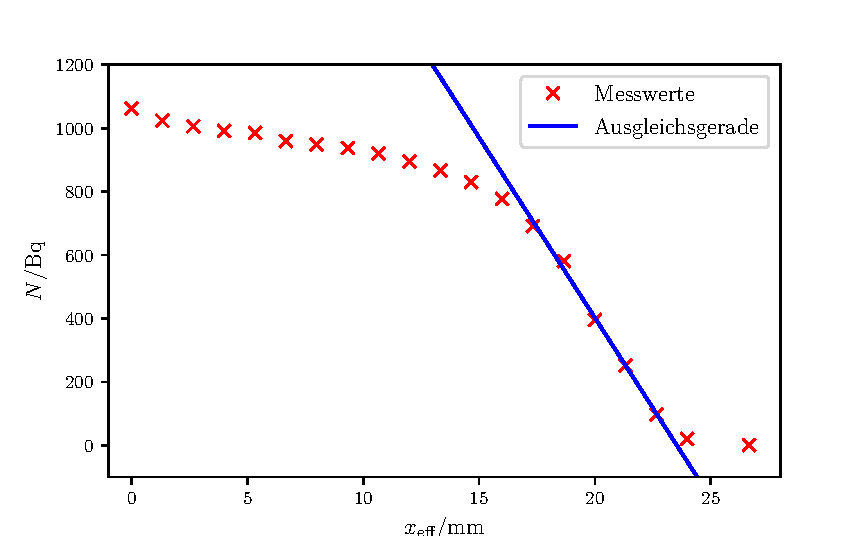
\includegraphics[width=\linewidth-70pt,height=\textheight-70pt,keepaspectratio]{content/images/Graph1N.pdf}
	\label{fig:1N}
\end{figure}
\begin{figure}
	\centering
	\caption{Die Energie $E_1$ aufgetragen gegen die effektive Länge $x_.{eff1}$.}
	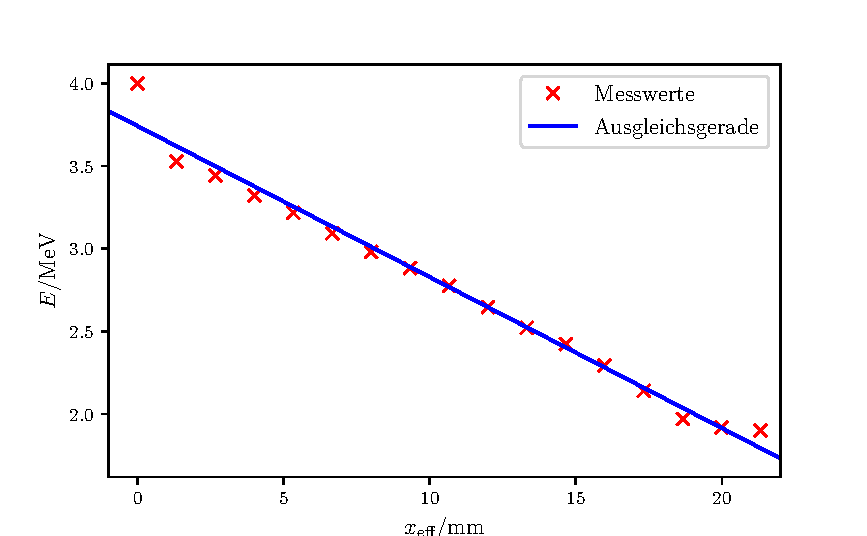
\includegraphics[width=\linewidth-70pt,height=\textheight-70pt,keepaspectratio]{content/images/Graph1E.pdf}
	\label{fig:1E}
\end{figure}

\subsection{Bestimmung der Reichweite von Alpha-Strahlung Messung 2}

\begin{table}
	\centering
	\caption{Der Druck $p$ und die Impulsrate $N_2$, sowie die effektiven Längen $x_.{eff2}$ und die bestimmten Energien $E_2$ bei der zweiten Messreihe mit einem Abstand zur Probe von $\SI{1}{\centi\metre}$.}
	\label{tab:tab2}
	\sisetup{table-format=1.2}
	\begin{tabular}{S[table-format=1.2]S[table-format=2.0]}
		\toprule
		{$\Delta p/\si{\bar}$} & {$N$} \\
		\midrule
		0.80 & 39 \\
		0.80 & 30 \\
		0.80 & 33 \\
		0.80 & 33 \\
		0.80 & 33 \\
		0.80 & 34 \\
		0.80 & 33 \\
		0.80 & 33 \\
		\bottomrule
	\end{tabular}

	\label{tab:2}
\end{table}
\begin{figure}
	\centering
	\caption{Die Impulsrate $N_2$ aufgetragen gegen die effektive Länge $x_.{eff2}$.}
	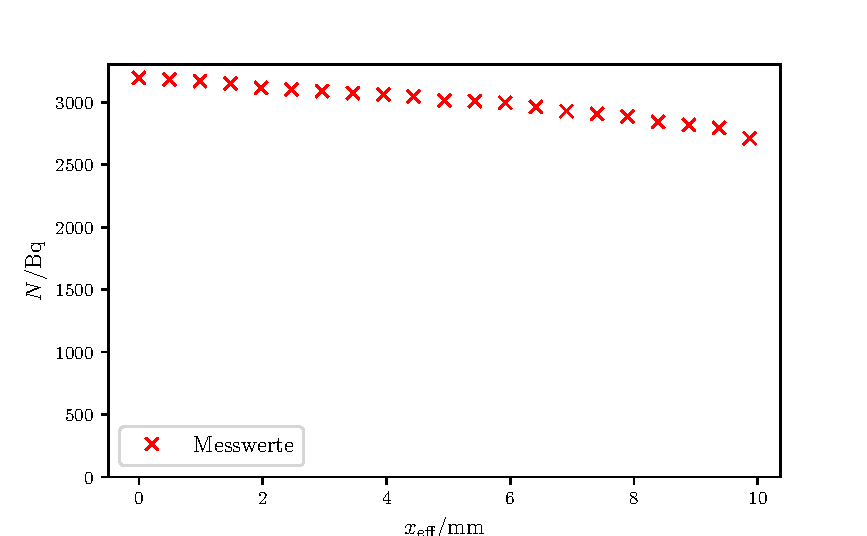
\includegraphics[width=\linewidth-70pt,height=\textheight-70pt,keepaspectratio]{content/images/Graph2N.pdf}
	\label{fig:2N}
\end{figure}
\begin{figure}
	\centering
	\caption{Die Energie $E_2$ aufgetragen gegen die effektive Länge $x_.{eff2}$.}
	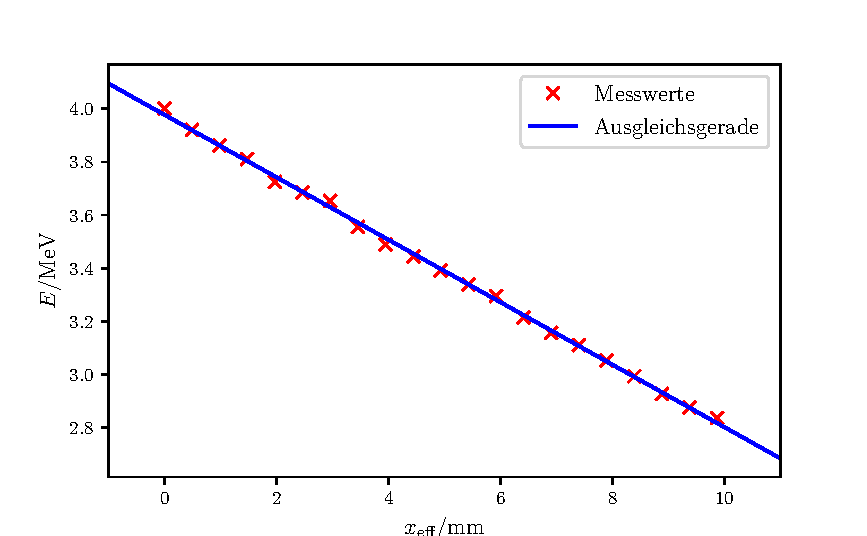
\includegraphics[width=\linewidth-70pt,height=\textheight-70pt,keepaspectratio]{content/images/Graph2E.pdf}
	\label{fig:2E}
\end{figure}

\subsection{Statistik des Radioaktiven Zerfalls}

\begin{figure}
	\centering
	\caption{Die normierte Häufigkeit aufgetragen gegen die Impulsrate $N$, sowie die zugehörige Poisson- und Gaußverteilung bei einem $\Delta N$ von 20.}
	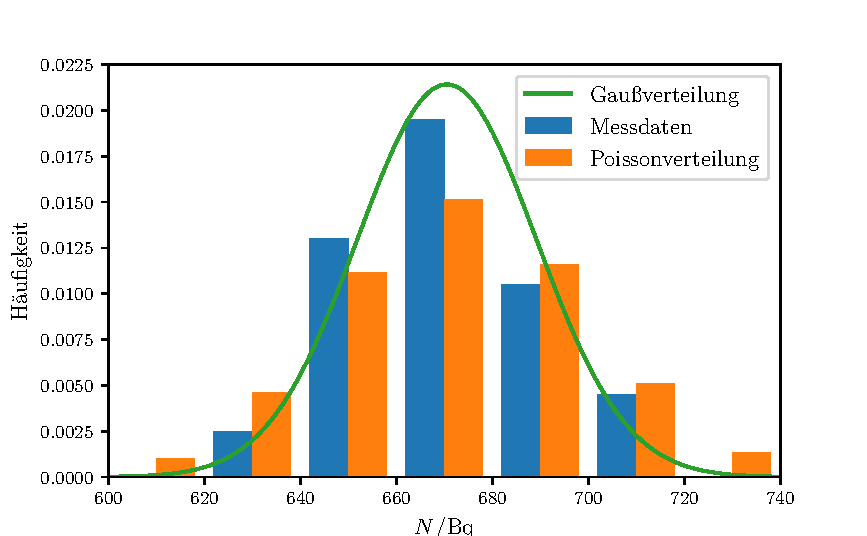
\includegraphics[width=\linewidth-70pt,height=\textheight-70pt,keepaspectratio]{content/images/Graph3_20.pdf}
	\label{fig:3_20}
\end{figure}
\begin{figure}
	\centering
	\caption{Die normierte Häufigkeit aufgetragen gegen die Impulsrate $N$, sowie die zugehörige Poisson- und Gaußverteilung bei einem $\Delta N$ von 10.}
	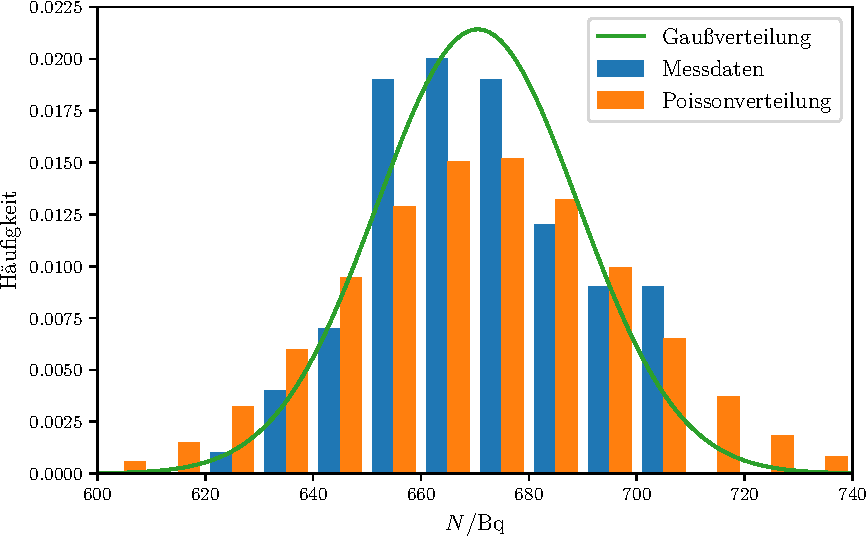
\includegraphics[width=\linewidth-70pt,height=\textheight-70pt,keepaspectratio]{content/images/Graph3_10.pdf}
	\label{fig:3_10}
\end{figure}
\begin{figure}
	\centering
	\caption{Die normierte Häufigkeit aufgetragen gegen die Impulsrate $N$, sowie die zugehörige Poisson- und Gaußverteilung bei einem weiteren $\Delta N$.}
	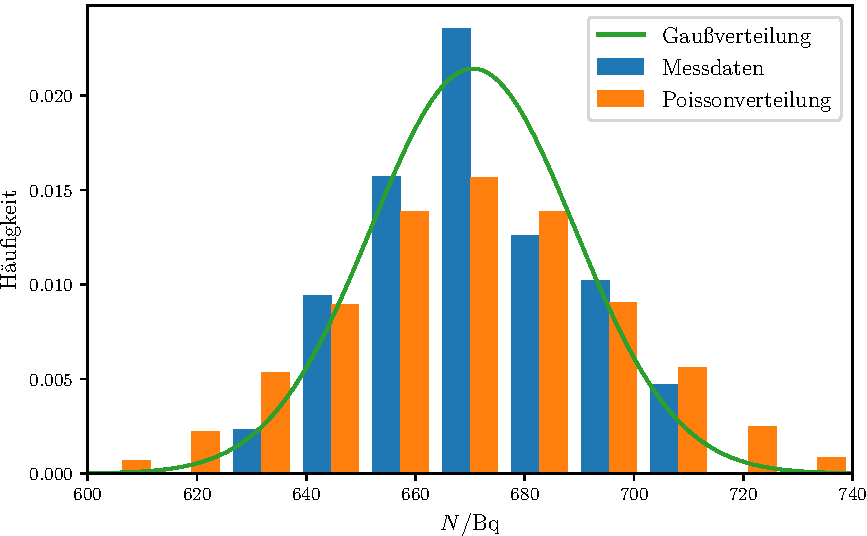
\includegraphics[width=\linewidth-70pt,height=\textheight-70pt,keepaspectratio]{content/images/Graph3_scott.pdf}
	\label{fig:3_scott}
\end{figure}
